\documentclass[text05.tex]{subfiles}
\begin{document}
\subsection{その他}
\subsubsection{有機ELディスプレイ}\label{oled}
\begin{table}[H]
	\begin{widerrows}
		\begin{tabular}{|p{\colF}|p{\colG}|}	\hline
		\ruby{名称}{めい|しょう} & 有機ELディスプレイ（ゆうきいーえるでぃすぷれい）\\ \hline
		\ruby{接続箇所}{せつ|ぞく|か|しょ} & I2C (4pin)\\ \hline
		\ruby{機能概要}{き|のう|がい|よう} & 文字の\ruby{表示}{ひょう|じ}\\ \hline
		\end{tabular}
  \end{widerrows}	
\end{table}

\begin{table}[H]
	\begin{widerrows}
		\begin{tabular}{|p{\colF}|p{\colG}|}	\hline
		サンプルコードの場所 & 05/oled.hsp\\ \hline
		raspiへの入力 & なし\\ \hline
		raspiへの入力方法 & なし\\ \hline
		raspiからの出力 & プログラムで決めた文字や記号を\ruby{表示}{ひょう|じ}する\\ \hline
		raspiからの出力方法 & oled “\ruby{表示}{ひょう|じ}させたい文字”\\ \hline
		\end{tabular}
  \end{widerrows}	
\end{table}

\begin{table}[H]
	\begin{widerrows}
		\begin{tabular}{|p{\colF}|p{\colG}|} \hline
		使い道 & テレビ\\ \hline
		\ruby{注意事項}{ちゅう|い|じ|こう} & 日本語\ruby{表示}{ひょう|じ}させることはできないので注意\\ \hline
		\ruby{補足}{ほ|そく} & なし\\ \hline
		\end{tabular}
  \end{widerrows}	
\end{table}

\begin{figure}[H]
	\begin{widerrows}
		\begin{tabular}{|p{\colH}|p{\colI}|p{\colH}|p{\colI}|} \hline
		外観 & 
		\begin{minipage}[t]{\linewidth}
			\smallskip
				\centering
				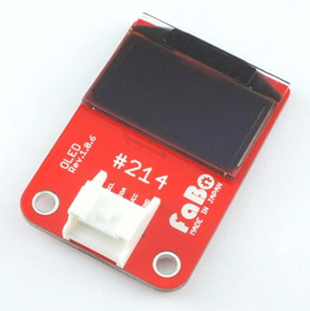
\includegraphics[width=0.5\linewidth]{../../asset/image/text05-img032.png}
				\caption{有機ELディスプレイ}
				\smallskip
			\end{minipage} &
			回路記号 & なし\\ \hline
		\end{tabular}
  \end{widerrows}	
\end{figure}
\end{document}
